\section{Modified Minimized Design}
From the S-parameter measurements of both the triangle feed antenna and the minimized monopole antenna, it is clear that both antennas are experiencing problems in the high band when moved from simulation to the PCB with tuner.

It has been chosen to elaborate on the minimized monopole antenna design and improve the high band. In order to do so, a second set of arms has been added to the antennas as shown in Figure~\ref{fig:sparam_5mm_highband}. As previous experience has shown that the simplified simulations will detune in practice, the matching components in Figure~\ref{fig:sparam_5mm_highband} have been chosen to resonate slightly higher than desired. 

\begin{figure}[htbp]
    \begin{subfigure}[t]{0.49\linewidth}
        \centering
        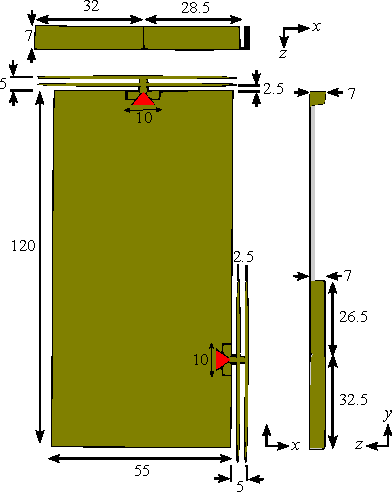
\includegraphics{img/tech_sol/monopole/highband/3d_drawing}
        \caption{Technical drawing.}
        \label{fig:ant1technical_highband}
    \end{subfigure}
    \hfill
    \begin{subfigure}[t]{0.49\linewidth}
        \centering
        \includegraphics{img/tech_sol/schematic_tuning_1}\\[1cm]
\footnotesize
        \begin{tabular}{|l|l|l|l|}
            \hline
            & $C_1$ & $L_1$ & $C_2$ \\
            \hline
            Top antenna & \SI{3.02}{pF} & \SI{7.99}{nH} & $[0.3,2.9]\,$pF\\
            Side antenna & \SI{1.81}{pF} & \SI{5.27}{nH} & $[0.3,2.9]\,$pF\\
            \hline
        \end{tabular}
        \caption{Tuning/matching circuit.}
        \label{fig:ant1_tuning_highband}
    \end{subfigure}
    \caption{Technical drawing and tuning circuit for the antenna. The matching circuit is applied for both the top and the side antenna.}
    \label{fig:sparam_5mm_highband}
\end{figure}

\FloatBarrier
\subsection{Simulation}
\label{sec:highbandsimulations}

\fixme{Finish this section, bandwidth table, write about corr and eff.}

The new antenna design presented in Figure~\ref{fig:sparam_5mm_highband} has been simulated. The resulting S-parameter sweep can be seen in Figure~\ref{fig:sparam_mono_modi_sim}. The low band of both antennas can be covered by sweeping the tuning capacitor. The high band resonates higher than desired but is likely to detune when the antennas are added to the PCB. The maximum bandwidth for both antennas can be seen in Table \ref{tab:bw_mono_modi_fs}. Both antennas covers the required bandwidth in the low band, but experiences some problems in the high band. The top antenna lacks \SI{393}{MHz} and the side antenna \SI{515}{MHz}. As a side effect of the extra added resonans the bandwidth have dropped. It should however be able to cover both bands  

sideeffect
The correlation sweep results can be seen in Figure \ref{fig:corr_mono_modi_sim_free}. The Efficiency sweep results can be seen in Figure \ref{fig:eff_mono_modi_sim_free}.


\begin{table}[htbp]
  \centering
  \begin{tabular}{|l|l|r|r|r|}
    \hline
    Antenna & Band & Start [MHz] & Stop [MHz] & Bandwidth [MHz] \\
    \hline
    Top     & Low  &  938  & 1065  & 127 \\
    Side    & Low  &  933  & 1031  & 98  \\
    \hline
    Top     & High &  2291 &  2218  & 327 \\
    Side    & High & 2128 &  2433 & 205 \\
    \hline
  \end{tabular}
  \caption{Monopole antenna in data mode. Maximum bandwidth obtained in the low and high band for the top and the side antenna, respectively.}    
  \label{tab:bw_mono_modi_fs}
\end{table}


% Sweeping S-parameters
\begin{figure}[htbp]
   \begin{subfigure}[b]{0.49\linewidth}
        \centering
        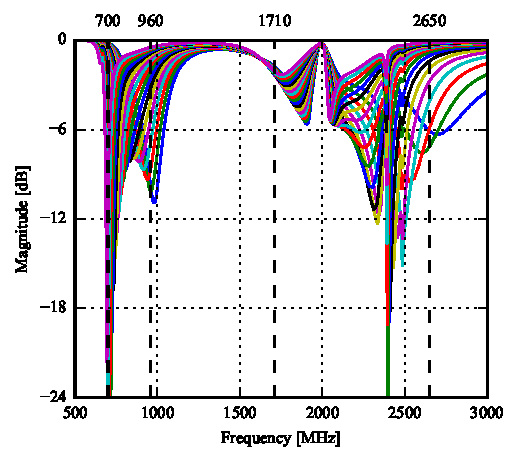
\includegraphics{img/tech_sol/monopole/highband/sim/s11.pdf}
        \caption{$S_{11}$, sweeping $C_1$ and fixing $C_2$.}
   \end{subfigure}
    \hfill
    \begin{subfigure}[b]{0.49\linewidth}
        \centering
        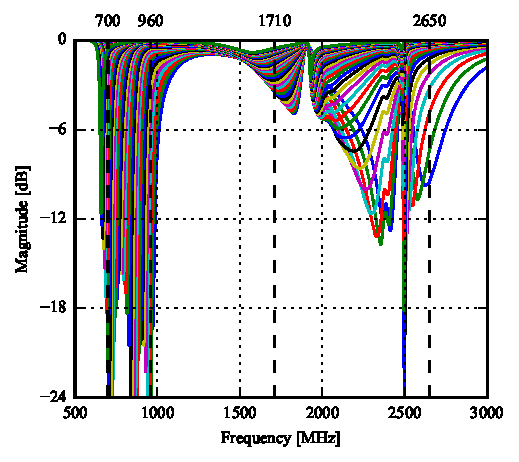
\includegraphics{img/tech_sol/monopole/highband/sim/s22.pdf}
        \caption{$S_{22}$, sweeping $C_2$ and fixing $C_1$.}
    \end{subfigure}
~
    \begin{subfigure}[b]{0.49\linewidth}
        \centering
        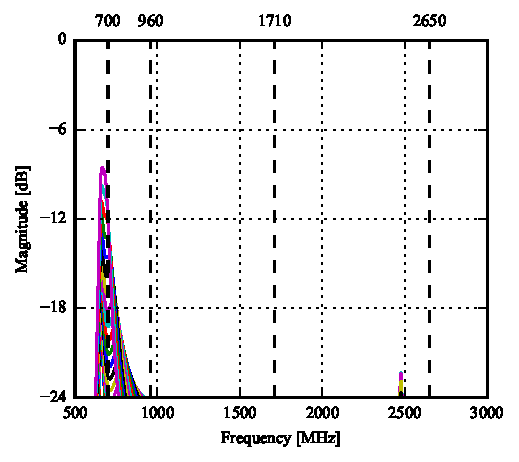
\includegraphics{img/tech_sol/monopole/highband/sim/s11_s21.pdf}
        \caption{$S_{21}$, sweeping $C_1$ and fixing $C_2$.}
    \end{subfigure}
    \hfill
    \begin{subfigure}[b]{0.49\linewidth}
        \centering
        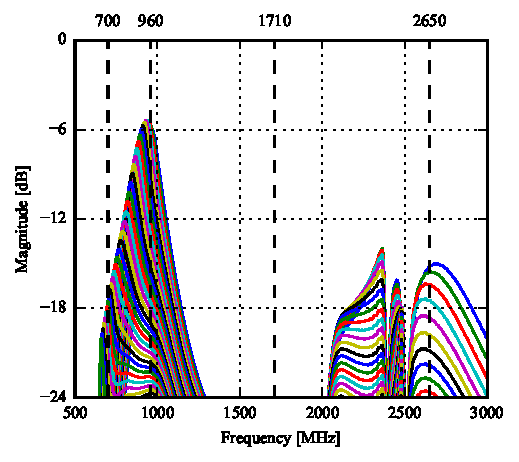
\includegraphics{img/tech_sol/monopole/highband/sim/s22_s21.pdf}
        \caption{$S_{21}$, sweeping $C_2$ and fixing $C_1$.}
    \end{subfigure}
    \caption{S-parameter sweep in free space for tuning the shunt capacitor of each antenna, $C_1$ and $C_2$ for port 1 and 2, respectively. Port 1 is the top antenna and port 2 is the side antenna.}
    \label{fig:sparam_mono_modi_sim}
\end{figure}

% Correlation
\begin{figure}[htbp]
    \centering
    \begin{subfigure}{0.49\linewidth}
      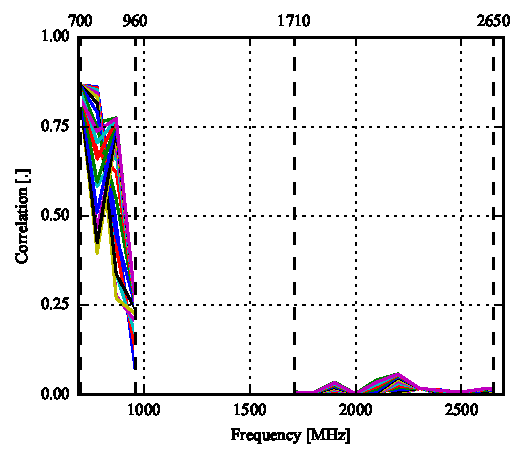
\includegraphics{img/tech_sol/monopole/highband/sim/corr_top.pdf}
        \caption{Sweeping $C_1$ and fixing $C_2$.}
    \end{subfigure}
    \hfill
    \begin{subfigure}{0.49\linewidth}
        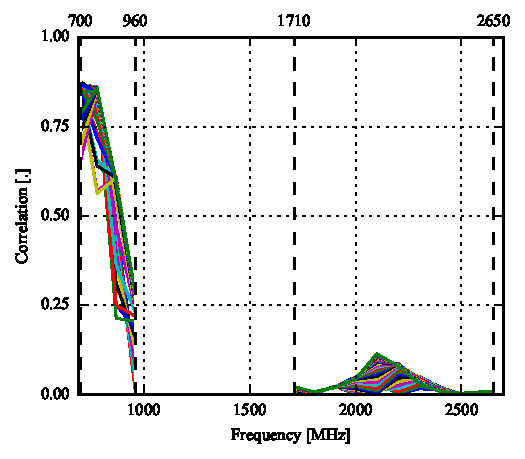
\includegraphics{img/tech_sol/monopole/highband/sim/corr_side.pdf}
        \caption{Sweeping $C_2$ and fixing $C_1$.}
    \end{subfigure}
    \caption{Correlation between antennas when sweeping tuning capacitors. Here, $C_1$ and $C_2$ are the tuning capacitor for the top and side antenna, respectively.}
    \label{fig:corr_mono_modi_sim_free}
\end{figure}

\begin{figure}[htbp]
    \centering
    \begin{subfigure}{0.49\linewidth}
        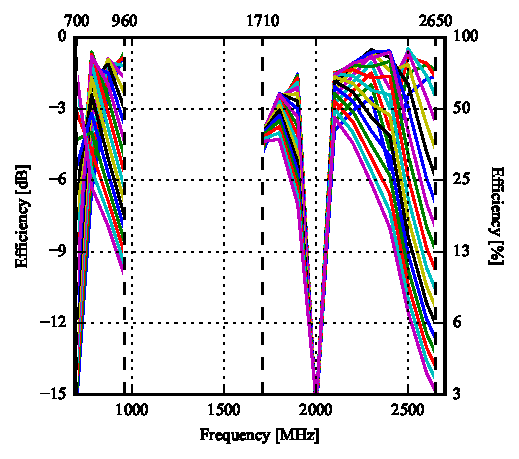
\includegraphics{img/tech_sol/monopole/highband/sim/eff_top.pdf}
        \caption{Sweeping $C_1$ and fixing $C_2$.}
    \end{subfigure}
    \hfill
    \begin{subfigure}{0.49\linewidth}
        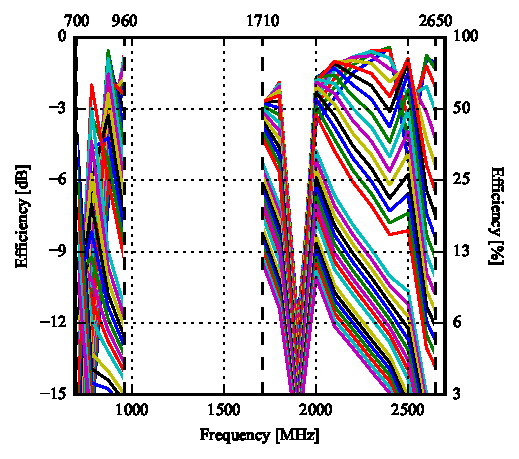
\includegraphics{img/tech_sol/monopole/highband/sim/eff_side.pdf}
        \caption{Sweeping $C_2$ and fixing $C_1$.}
    \end{subfigure}
    \caption{Efficiency for each antenna when sweeping the tunable capacitors. Here, $C_1$ and $C_2$ are the tuning capacitor for the top and side antenna, respectively.}
    \label{fig:eff_mono_modi_sim_free}
\end{figure}

\FloatBarrier
\subsection{User Effect Simulations}
In this section the modified monopole antenna will be simulated in pratice use with an user. The antenna position for each simulation is shown in Figure \ref{fig:position_mono_modi}.

\begin{figure}[htbp]
    \centering
    \begin{subfigure}[b]{0.24\linewidth}
        \centering 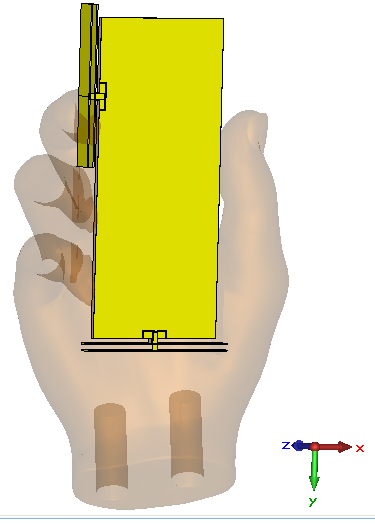
\includegraphics[width=\linewidth,height=4cm,keepaspectratio]{img/tech_sol/monopole/highband/ue/datamode/3d_datamode.PNG}
        \caption{Data mode.}
    \end{subfigure}
    \begin{subfigure}[b]{0.24\linewidth}
        \centering 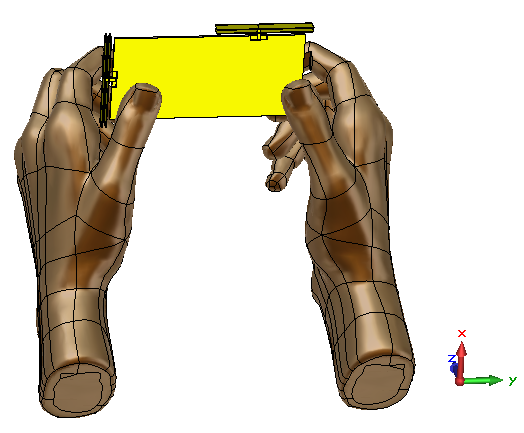
\includegraphics[width=\linewidth,height=4cm,keepaspectratio]{img/tech_sol/monopole/highband/ue/playmode/3d_playmode.PNG}
        \caption{Play mode.}
    \end{subfigure}
    \begin{subfigure}[b]{0.24\linewidth}
        \centering 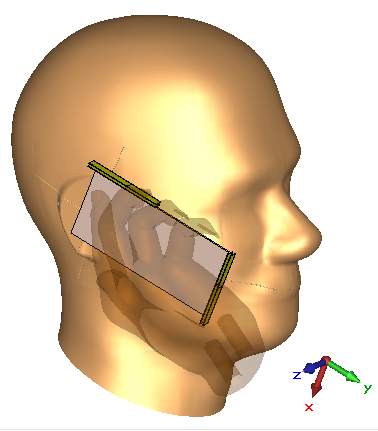
\includegraphics[width=\linewidth,height=4cm,keepaspectratio]{img/tech_sol/monopole/highband/ue/talkmode/3d_talkmode.PNG}
        \caption{Talk mode.}
    \end{subfigure}
    \begin{subfigure}[b]{0.24\linewidth}
        \centering 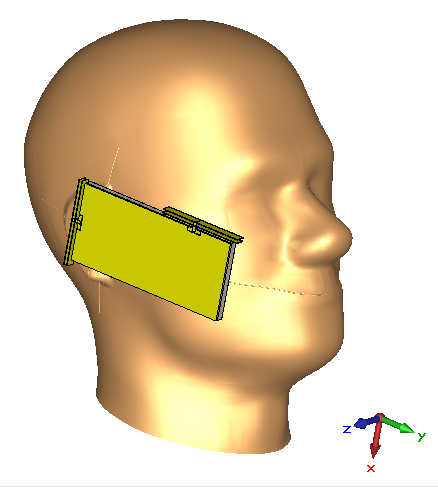
\includegraphics[width=\linewidth,height=4cm,keepaspectratio]{img/tech_sol/monopole/highband/ue/sar/3d_sar.PNG}
        \caption{SAR.}
    \end{subfigure}
    \caption{MIMO monopole antenna position for each user effect simulation.}
    \label{fig:position_mono_modi}
\end{figure}

\fixme{S-parameter plot, bandwidth table and documentation for all positions.}
\FloatBarrier
\subsubsection{Data Mode}

\begin{table}[htbp]
  \centering
  \begin{tabular}{|l|l|r|r|r|}
    \hline
    Antenna & Band & Start [MHz] & Stop [MHz] & Bandwidth [MHz] \\
    \hline
    Top     & Low  &  677  & 1065  & 388 \\
    Side    & Low  &  700  & 710  & 10  \\
    \hline
    Top     & High &  1183 &  2127  & 944 \\
    Side    & High & 1765 &  2120 & 355 \\
    \hline
  \end{tabular}
  \caption{Monopole antenna in data mode. Maximum bandwidth obtained in the low and high band for the top and the side antenna, respectively.}    
  \label{tab:bw_mono_modi_dm}
\end{table}
%S-Parameters
The S-parameter sweeps can be seen in Figure \ref{fig:sparam_mono_modi_data_mode}.

%Correlation
The correlation between the top and side antenna can be seen in Figure \ref{fig:corr_mono_modi_data_mode}.
%Efficiency
The Efficiency sweep can be seen in Figure \ref{fig:eff_mono_modi_data_mode}. 
%S-Parameter
\begin{figure}[htbp]
   \begin{subfigure}[b]{0.49\linewidth}
        \centering
        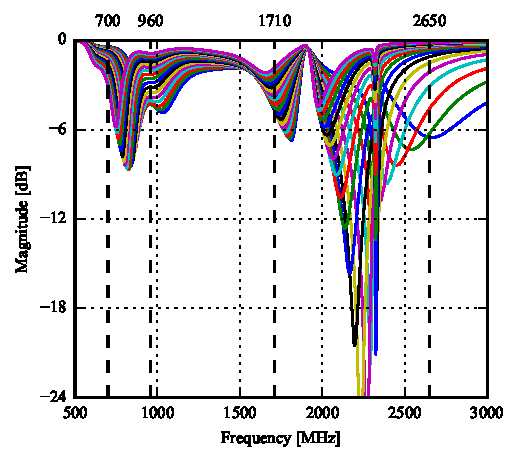
\includegraphics{img/tech_sol/monopole/highband/ue/datamode/s11.pdf}
        \caption{$S_{11}$, sweeping $C_1$ and fixing $C_2$.}
    \end{subfigure}
    \hfill
    \begin{subfigure}[b]{0.49\linewidth}
        \centering
        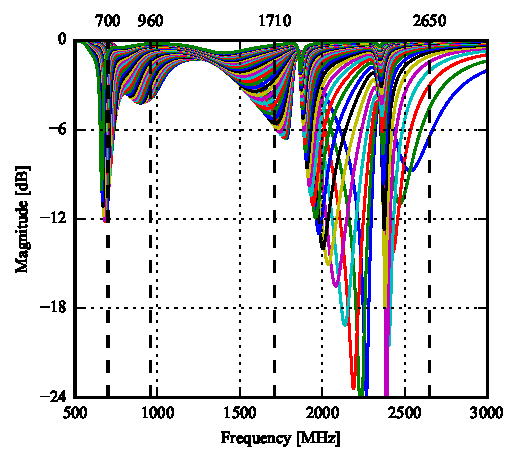
\includegraphics{img/tech_sol/monopole/highband/ue/datamode/s22.pdf}
        \caption{$S_{22}$, sweeping $C_2$ and fixing $C_1$.}
    \end{subfigure}
~
    \begin{subfigure}[b]{0.49\linewidth}
        \centering
        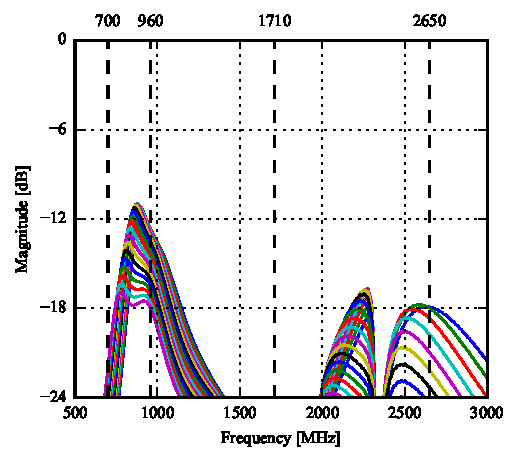
\includegraphics{img/tech_sol/monopole/highband/ue/datamode/s12.pdf}
        \caption{$S_{21}$, sweeping $C_1$ and fixing $C_2$.}
    \end{subfigure}
    \hfill
    \begin{subfigure}[b]{0.49\linewidth}
        \centering
        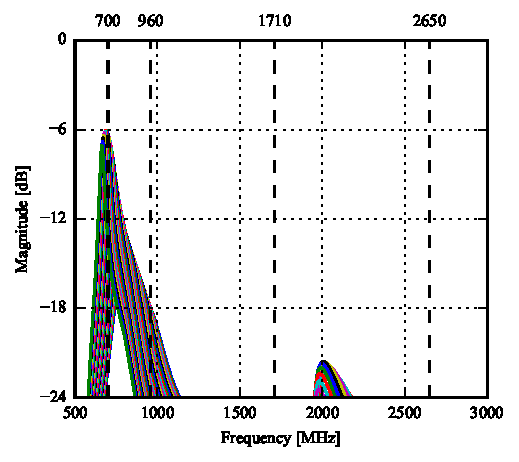
\includegraphics{img/tech_sol/monopole/highband/ue/datamode/s21.pdf}
        \caption{$S_{21}$, sweeping $C_2$ and fixing $C_1$.}
    \end{subfigure}
    \caption{S-parameter sweep in data mode for tuning the shunt capacitor of each antenna, $C_1$ and $C_2$ for port 1 and 2, respectively. Port 1 is the top antenna and port 2 is the side antenna.}
    \label{fig:sparam_mono_modi_data_mode}
\end{figure}

%Correlation
\begin{figure}[htbp]
    \centering
    \begin{subfigure}{0.49\linewidth}
        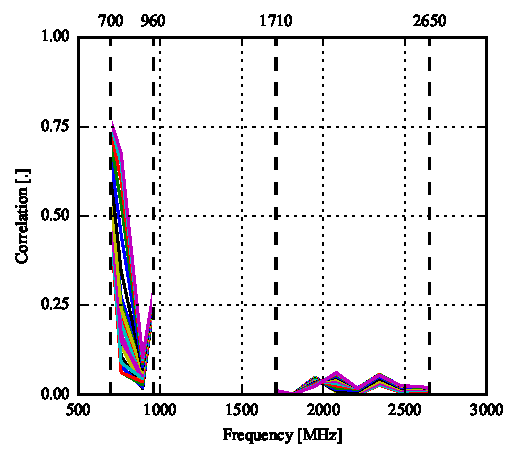
\includegraphics{img/tech_sol/monopole/highband/ue/datamode/corr_top.pdf}
        \caption{Sweeping $C_1$ and fixing $C_2$.}
    \end{subfigure}
    \hfill
    \begin{subfigure}{0.49\linewidth}
        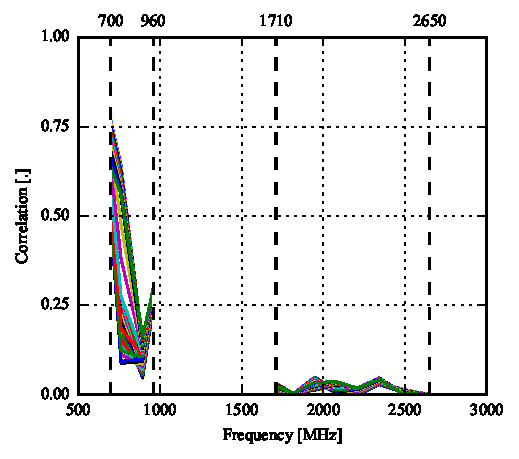
\includegraphics{img/tech_sol/monopole/highband/ue/datamode/corr_side.pdf}
        \caption{Sweeping $C_2$ and fixing $C_1$.  \fixme{replace top with side correlation}}
    \end{subfigure}
    \caption{Monopole antenna in data mode. Correlation between antennas when sweeping tuning capacitors. Here, $C_1$ and $C_2$ are the tuning capacitor for the top and side antenna, respectively.}
    \label{fig:corr_mono_modi_data_mode}
\end{figure}


%Efficiency
\begin{figure}[htbp]
    \centering
    \begin{subfigure}{0.49\linewidth}
        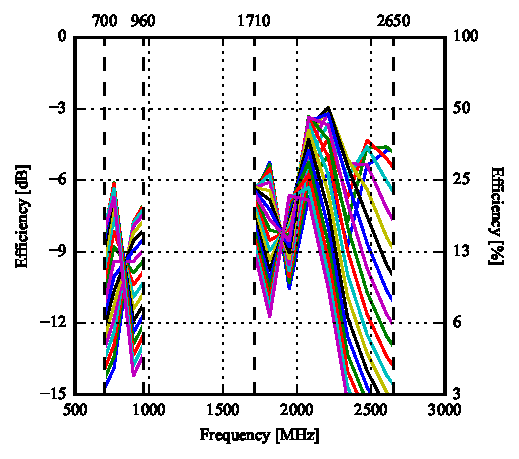
\includegraphics{img/tech_sol/monopole/highband/ue/datamode/eff_top.pdf}
        \caption{Sweeping $C_1$ and fixing $C_2$.}
    \end{subfigure}
    \hfill
    \begin{subfigure}{0.49\linewidth}
        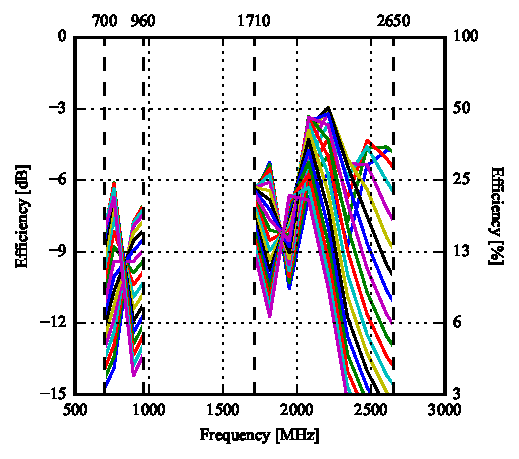
\includegraphics{img/tech_sol/monopole/highband/ue/datamode/eff_top.pdf}
        \caption{Sweeping $C_2$ and fixing $C_1$.}
    \end{subfigure}
    \caption{Monopole antenna in data mode. Efficiency for each antenna when sweeping the tunable capacitors. Here, $C_1$ and $C_2$ are the tuning capacitor for the top and side antenna, respectively.}
    \label{fig:eff_mono_modi_data_mode}
\end{figure}

\FloatBarrier
\subsubsection{Play Mode}

\begin{table}[htbp]
  \centering
  \begin{tabular}{|l|l|r|r|r|}
    \hline
    Antenna & Band & Start [MHz] & Stop [MHz] & Bandwidth [MHz] \\
    \hline
    Top     & Low  &  677  & 1065  & 388 \\
    Side    & Low  &  700  & 710  & 10  \\
    \hline
    Top     & High &  1183 &  2127  & 944 \\
    Side    & High & 1765 &  2120 & 355 \\
    \hline
  \end{tabular}
  \caption{Monopole antenna in data mode. Maximum bandwidth obtained in the low and high band for the top and the side antenna, respectively.}    
  \label{tab:bw_mono_modi_pm}
\end{table}

%S-Parameters
The S-parameter sweeps can be seen in Figure \ref{fig:sparam_mono_modi_play_mode}.

%Correlation
The correlation between the top and side antenna can be seen in Figure \ref{fig:corr_mono_modi_play_mode}.
%Efficiency
The Efficiency sweep can be seen in Figure \ref{fig:eff_mono_modi_play_mode}. 
%S-Parameter
  \begin{figure}[htbp]
    \begin{subfigure}[b]{0.49\linewidth}
      \centering
      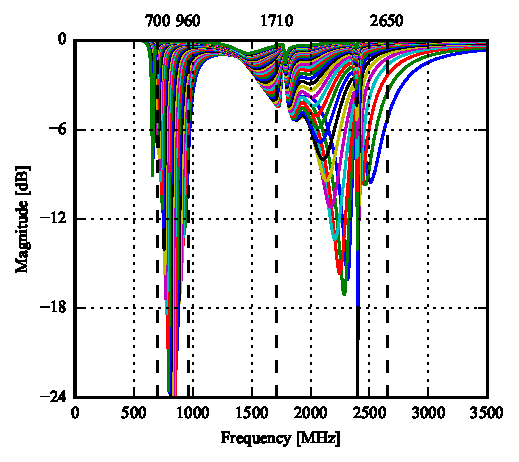
\includegraphics{img/tech_sol/monopole/highband/ue/playmode/s11.pdf}
      \caption{$S_{11}$, sweeping $C_1$ and fixing $C_2$.}
    \end{subfigure}
    \hfill
    \begin{subfigure}[b]{0.49\linewidth}
        \centering
        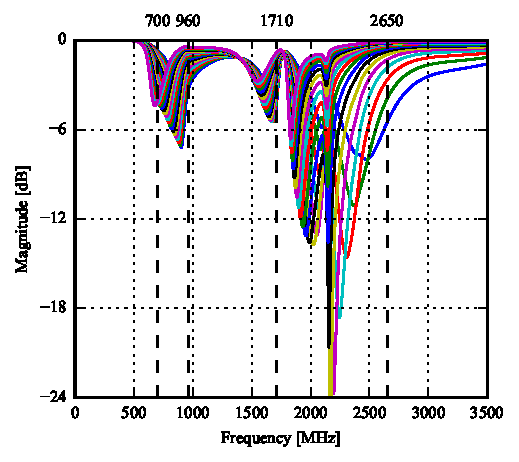
\includegraphics{img/tech_sol/monopole/highband/ue/playmode/s22.pdf}
        \caption{$S_{22}$, sweeping $C_2$ and fixing $C_1$.}
    \end{subfigure}
~
    \begin{subfigure}[b]{0.49\linewidth}
        \centering
        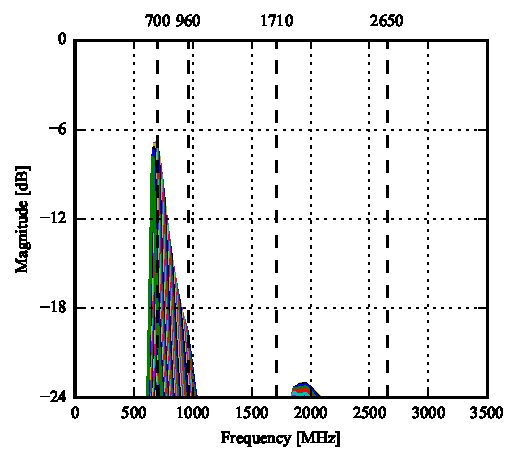
\includegraphics{img/tech_sol/monopole/highband/ue/playmode/s12.pdf}
        \caption{$S_{21}$, sweeping $C_1$ and fixing $C_2$.}
    \end{subfigure}
    \hfill
    \begin{subfigure}[b]{0.49\linewidth}
        \centering
        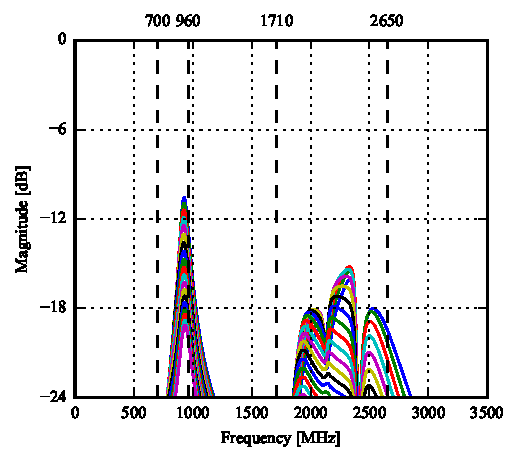
\includegraphics{img/tech_sol/monopole/highband/ue/playmode/s21.pdf}
        \caption{$S_{21}$, sweeping $C_2$ and fixing $C_1$.}
    \end{subfigure}
    \caption{S-parameter sweep in play mode for tuning the shunt capacitor of each antenna, $C_1$ and $C_2$ for port 1 and 2, respectively. Port 1 is the top antenna and port 2 is the side antenna.}
    \label{fig:sparam_mono_modi_play_mode}
\end{figure}

% Correlation
\begin{figure}[htbp]
    \centering
    \begin{subfigure}{0.49\linewidth}
        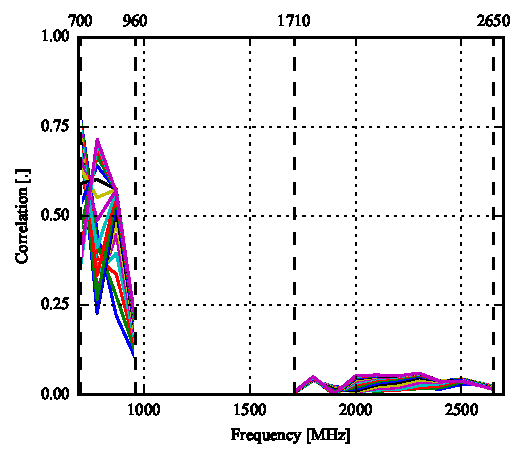
\includegraphics{img/tech_sol/monopole/highband/ue/playmode/corr_top.pdf}
        \caption{Sweeping $C_1$ and fixing $C_2$.}
    \end{subfigure}
    \hfill
    \begin{subfigure}{0.49\linewidth}
        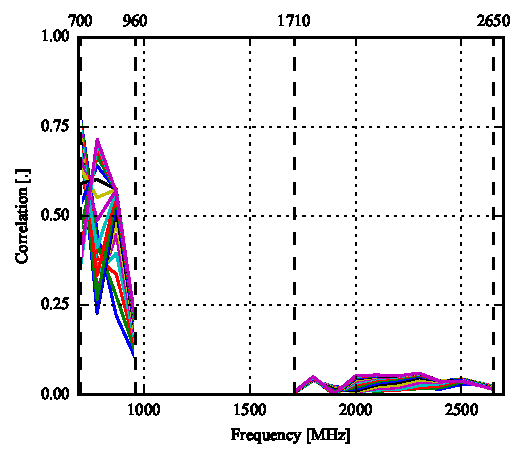
\includegraphics{img/tech_sol/monopole/highband/ue/playmode/corr_top.pdf}
        \caption{Sweeping $C_2$ and fixing $C_1$.}
    \end{subfigure}
    \caption{Monopole antenna in play mode. Correlation between antennas when sweeping tuning capacitors. Here, $C_1$ and $C_2$ are the tuning capacitor for the top and side antenna, respectively.}
    \label{fig:corr_mono_modi_play_mode}
\end{figure}

%Efficiency
\begin{figure}[htbp]
    \centering
    \begin{subfigure}{0.49\linewidth}
        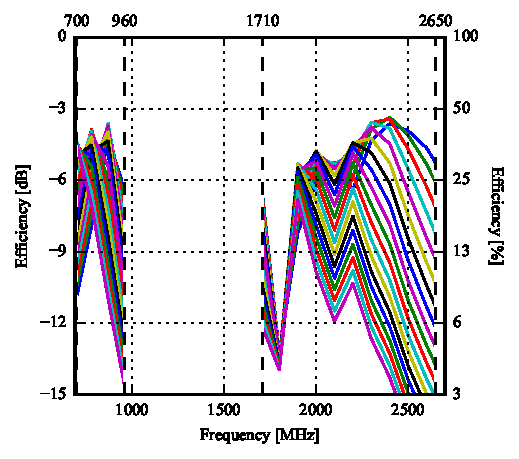
\includegraphics{img/tech_sol/monopole/highband/ue/playmode/eff_top.pdf}
        \caption{Sweeping $C_1$ and fixing $C_2$.}
    \end{subfigure}
    \hfill
    \begin{subfigure}{0.49\linewidth}
        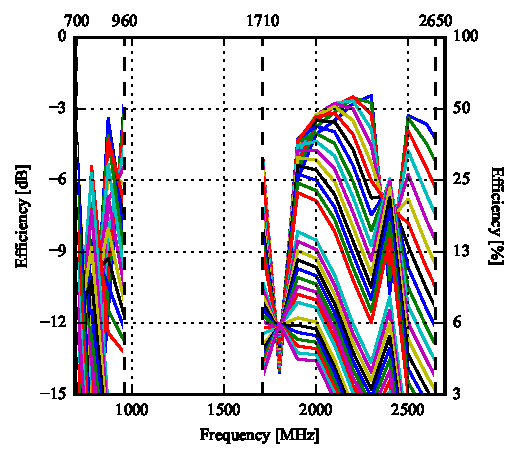
\includegraphics{img/tech_sol/monopole/highband/ue/playmode/eff_side.pdf}
        \caption{Sweeping $C_2$ and fixing $C_1$.}
    \end{subfigure}
    \caption{Monopole antenna in play mode. Efficiency for each antenna when sweeping the tunable capacitors. Here, $C_1$ and $C_2$ are the tuning capacitor for the top and side antenna, respectively.}
    \label{fig:eff_mono_modi_play_mode}
\end{figure}

\FloatBarrier
\subsubsection{Talk Mode}
\begin{table}[htbp]
  \centering
  \begin{tabular}{|l|l|r|r|r|}
    \hline
    Antenna & Band & Start [MHz] & Stop [MHz] & Bandwidth [MHz] \\
    \hline
    Top     & Low  &  677  & 1065  & 388 \\
    Side    & Low  &  700  & 710  & 10  \\
    \hline
    Top     & High &  1183 &  2127  & 944 \\
    Side    & High & 1765 &  2120 & 355 \\
    \hline
  \end{tabular}
  \caption{Monopole antenna in data mode. Maximum bandwidth obtained in the low and high band for the top and the side antenna, respectively.}    
  \label{tab:bw_mono_modi_tm}
\end{table}

%S-Parameters
The S-parameter sweeps can be seen in Figure \ref{fig:sparam_mono_modi_talk_mode}.

%Correlation
The correlation between the top and side antenna can be seen in Figure \ref{fig:corr_mono_modi_talk_mode}.
%Efficiency
The Efficiency sweep can be seen in Figure \ref{fig:eff_mono_modi_talk_mode}. 
%S-Parameter

% S-parameters
\begin{figure}[htbp]
   \begin{subfigure}[b]{0.49\linewidth}
        \centering
        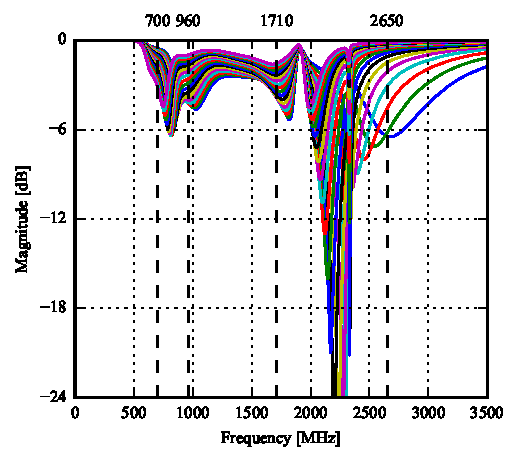
\includegraphics{img/tech_sol/monopole/highband/ue/talkmode/s11.pdf}
        \caption{$S_{11}$, sweeping $C_1$ and fixing $C_2$.}
    \end{subfigure}
    \hfill
    \begin{subfigure}[b]{0.49\linewidth}
        \centering
        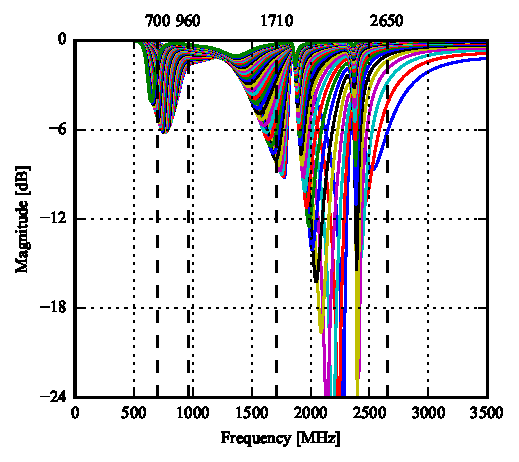
\includegraphics{img/tech_sol/monopole/highband/ue/talkmode/s22.pdf}
        \caption{$S_{22}$, sweeping $C_2$ and fixing $C_1$.}
    \end{subfigure}
~
    \begin{subfigure}[b]{0.49\linewidth}
        \centering
        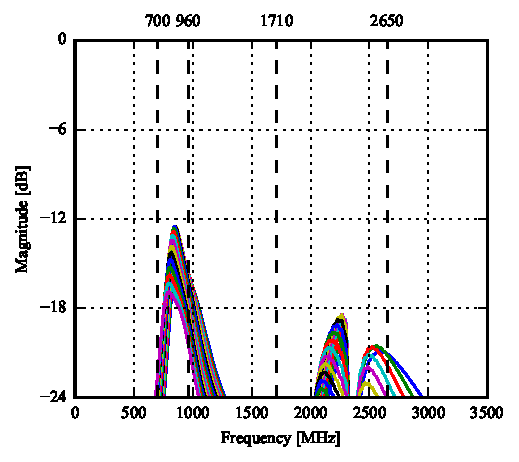
\includegraphics{img/tech_sol/monopole/highband/ue/talkmode/s12.pdf}
        \caption{$S_{21}$, sweeping $C_1$ and fixing $C_2$.}
    \end{subfigure}
    \hfill
    \begin{subfigure}[b]{0.49\linewidth}
        \centering
        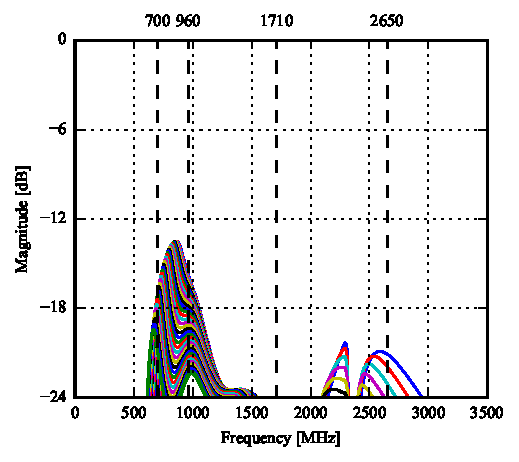
\includegraphics{img/tech_sol/monopole/highband/ue/talkmode/s21.pdf}
        \caption{$S_{21}$, sweeping $C_1$ and fixing $C_2$.}
    \end{subfigure}
    \caption{S-parameter sweep in talk mode for tuning the shunt capacitor of each antenna, $C_1$ and $C_2$ for port 1 and 2, respectively. Port 1 is the top antenna and port 2 is the side antenna.}
    \label{fig:sparam_mono_modi_talk_mode}
\end{figure}

% Correlation
\begin{figure}[htbp]
    \centering
    \begin{subfigure}{0.49\linewidth}
        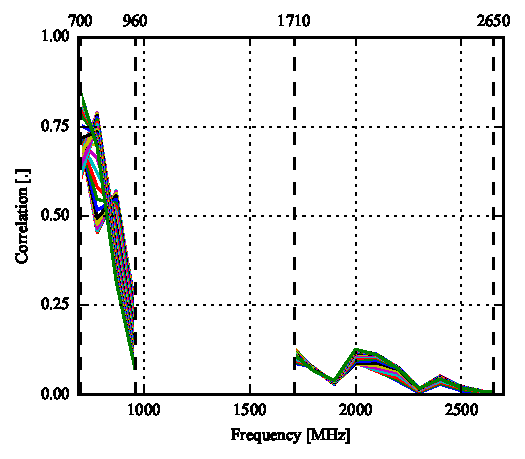
\includegraphics{img/tech_sol/monopole/highband/ue/talkmode/corr_top.pdf}
        \caption{Sweeping $C_1$ and fixing $C_2$.}
    \end{subfigure}
    \hfill
    \begin{subfigure}{0.49\linewidth}
        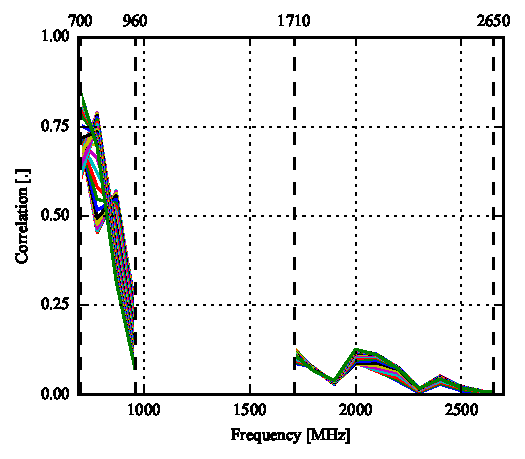
\includegraphics{img/tech_sol/monopole/highband/ue/talkmode/corr_side.pdf}
        \caption{Sweeping $C_2$ and fixing $C_1$.}
    \end{subfigure}
    \caption{Monopole antenna in talk mode. Correlation between antennas when sweeping tuning capacitors. Here, $C_1$ and $C_2$ are the tuning capacitor for the top and side antenna, respectively.}
    \label{fig:corr_mono_modi_talk_mode}
\end{figure}

%Efficiency
\begin{figure}[htbp]
    \centering
    \begin{subfigure}{0.49\linewidth}
        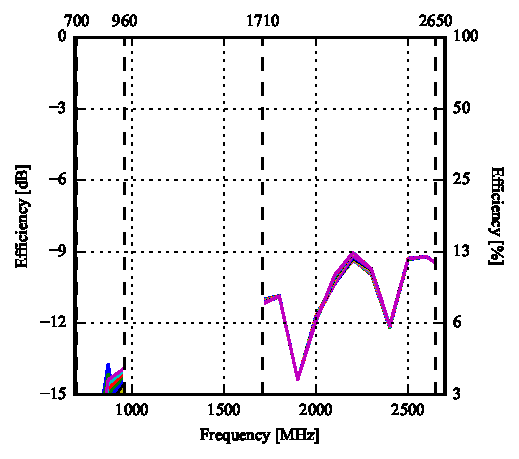
\includegraphics{img/tech_sol/monopole/highband/ue/talkmode/eff_top.pdf}
        \caption{Sweeping $C_1$ and fixing $C_2$.}
    \end{subfigure}
    \hfill
    \begin{subfigure}{0.49\linewidth}
        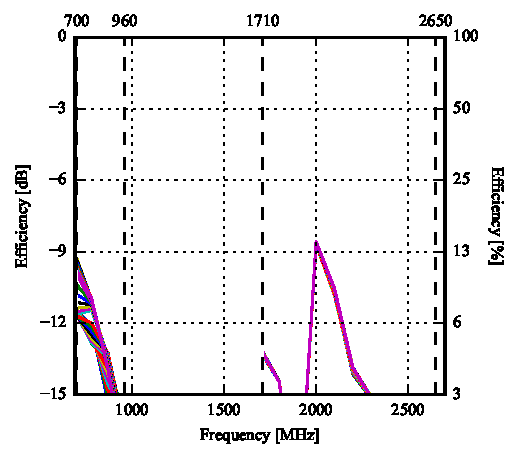
\includegraphics{img/tech_sol/monopole/highband/ue/talkmode/eff_side.pdf}
        \caption{Sweeping $C_2$ and fixing $C_1$.}
    \end{subfigure}
    \caption{Monopole antenna in talk mode. Efficiency for each antenna when sweeping the tunable capacitors. Here, $C_1$ and $C_2$ are the tuning capacitor for the top and side antenna, respectively.}
    \label{fig:eff_mono_modi_talk_mode}
\end{figure}

\FloatBarrier
\subsubsection{SAR}
The SAR simulation results can be seen in Figure \ref{fig:sar_mono_modi}. As seen from the figure the sar values for both the top and the side antenna fulfills the requirement. The top antenna has the highest SAR value of \SI{1.5}{W\per kg} in the high band and the side antenna has a maximum SAR value of \SI{0.6}{W\per kg} in the high band. 
\begin{figure}[htbp]
    \centering
    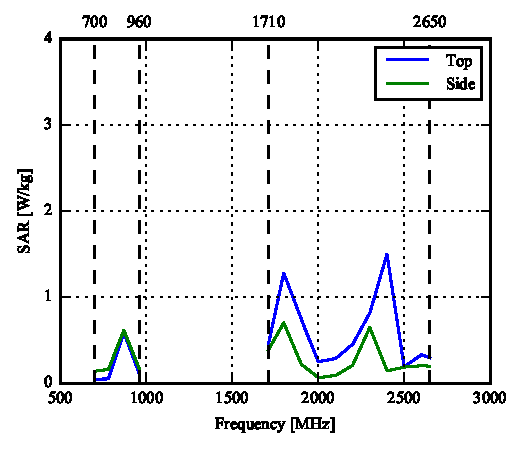
\includegraphics{img/tech_sol/monopole/highband/ue/sar/sar.pdf}
    \caption{SAR simulation of the monopole antenna.\fixme{new sar plot with screen}}
    \label{fig:sar_mono_modi}
\end{figure}

\FloatBarrier
\subsection{Measurements}
The antennas just simulated have been built and soldered onto the PCB described in the introduction. The component values for the matching network are shown in Figure~\ref{fig:mono_matching_modi_meas}. The measured S-parameters are shown in Figure~\ref{fig:sparam_mono_modi_meas}. When compared to the simulations in Section~\ref{sec:highbandsimulations}, it is seen that the antenna is indeed detunes as expected. However, the bandwidth is severely reduced and, even with different values for the matching network, the desired bandwidth at \SI{6}{dB} return loss could not be obtained.

In order to obtain better results, the transmission lines one the board has been modified for the final design and measurement. This will be described in the next section.

\begin{figure}[htbp]
        \centering
        \begin{tabular}{m{3in}m{3in}}
            \centering
            \includegraphics{img/tech_sol/schematic_tuning_1}&
            \centering
            \footnotesize
            \begin{tabular}{|l|l|l|l|}
                \hline
                & $C_1$ & $L_1$ & $C_2$ \\
                \hline
              Top antenna & \SI{3.9}{pF} & \SI{2.2}{nH} & \SI{0.6}{pF} \\
              Side antenna & \SI{4}{pF} & \SI{1}{nH} & \SI{1.2}{pF} \\
                \hline
            \end{tabular}
        \end{tabular}
    \caption{Matching circuit for the minimized monopole prototype. These are the component values where the bandwidth is found to be the largest.}
    \label{fig:mono_matching_modi_meas}
\end{figure}

\begin{figure}[htbp]
    \centering
    \begin{subfigure}{0.49\linewidth}
        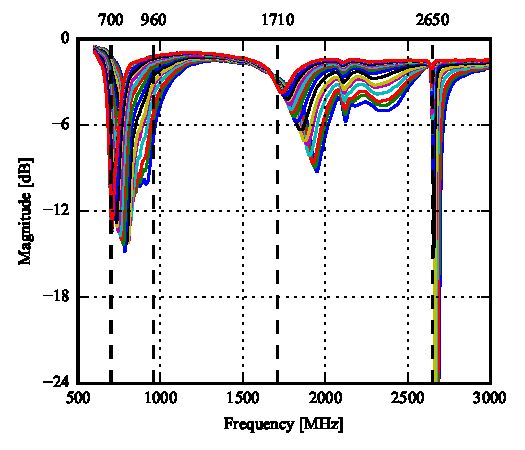
\includegraphics{img/tech_sol/monopole/highband/meas/tuner/S11.pdf}
        \caption{S11.}
    \end{subfigure}
    \hfill
    \begin{subfigure}{0.49\linewidth}
        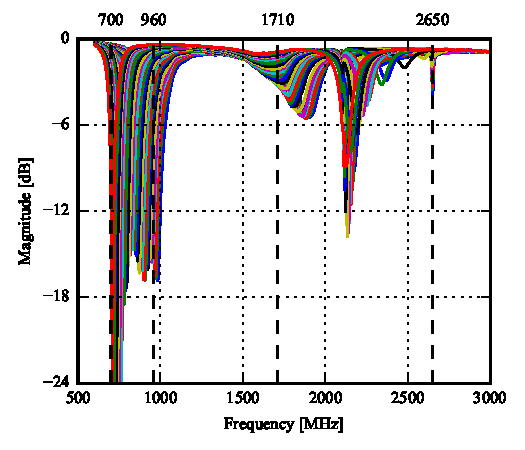
\includegraphics{img/tech_sol/monopole/highband/meas/tuner/S22.pdf}
        \caption{S22.}
    \end{subfigure}
    \\
    \begin{subfigure}{0.49\linewidth}
        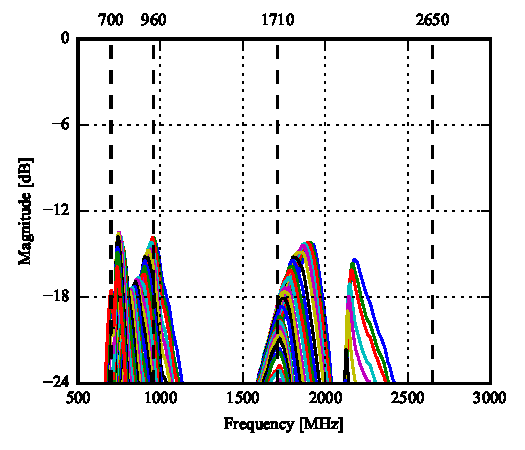
\includegraphics{img/tech_sol/monopole/highband/meas/tuner/S21.pdf}
        \caption{S21.}
    \end{subfigure}
    \caption{S-parameters for the modified minimized monopole prototype. The top-tuner is swept from approximately \SI{0.6}{pF} to \SI{6}{pF} and the side-tuner is swept from approximately \SI{1.2}{pF} to \SI{12}{pF}. The two tuners are tracking the first half of the sweep.}
    \label{fig:sparam_mono_modi_meas}
\end{figure}

\FloatBarrier
\subsection{Final Design and Measurements}
In this section, the final design with all above mentioned improvements will be presented. The design is shown in Figure~\ref{fig:final_lassedouble}, and dimensions of the antenna elements are the same as shown in Figure~\ref{fig:sparam_5mm_highband}. As shown in Figure~\ref{fig:final_lassedouble}, a capacitor has been added on each transmission line (from SMA to matching network), improving the return loss significantly. The matching network is nearly the same as in Figure~\ref{fig:mono_matching_modi_meas}. The exact component values are printed on Figure~\ref{fig:final_lassedouble}.

\begin{figure}[htbp]
    \centering
    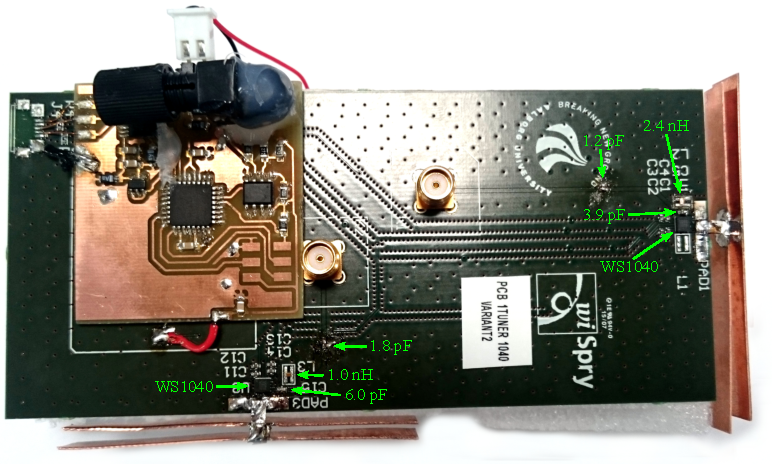
\includegraphics{img/tech_sol/monopole/highband/meas/final_tuner/lassedouble.pdf}
    \caption{Final antenna design with capacitors added to the transmission line to improve high-band performance.}
    \label{fig:final_lassedouble}
\end{figure}

\begin{figure}[htbp]
    \centering
    \begin{subfigure}{0.49\linewidth}
        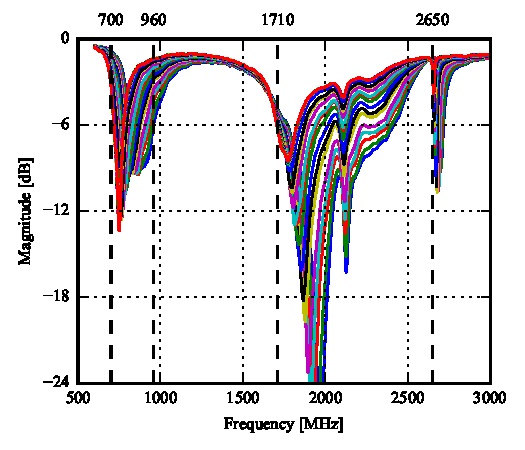
\includegraphics{img/tech_sol/monopole/highband/meas/final_tuner/S11.pdf}
        \caption{S11.}
    \end{subfigure}
    \hfill
    \begin{subfigure}{0.49\linewidth}
        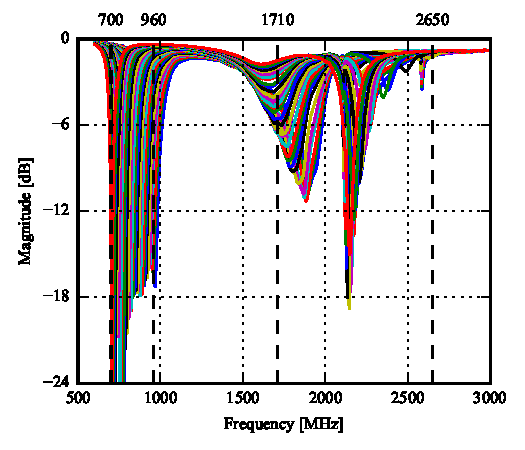
\includegraphics{img/tech_sol/monopole/highband/meas/final_tuner/S22.pdf}
        \caption{S22.}
    \end{subfigure}
    \\
    \begin{subfigure}{0.49\linewidth}
        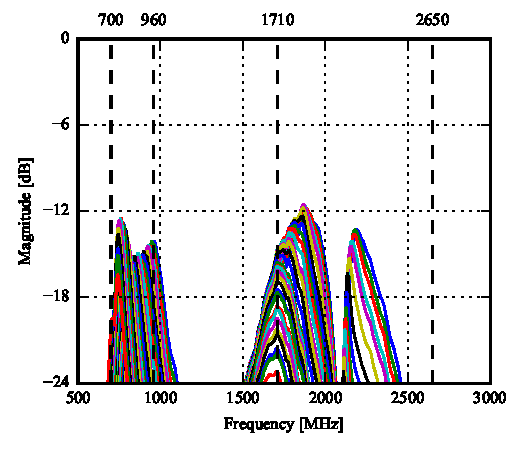
\includegraphics{img/tech_sol/monopole/highband/meas/final_tuner/S21.pdf}
        \caption{S21.}
    \end{subfigure}
    \caption{S-parameters of the final antenna design. The top antenna is swept from approximately \SI{0.6}{pF} to \SI{6}{pF} and the side antenna from approximately \SI{1.2}{pF} to \SI{12}{pF}. The tuners are tracking the first half of the sweep.} 
    \label{fig:final_sparams}
\end{figure}

\begin{figure}[htbp]
    \centering
    \begin{subfigure}{0.49\linewidth}
        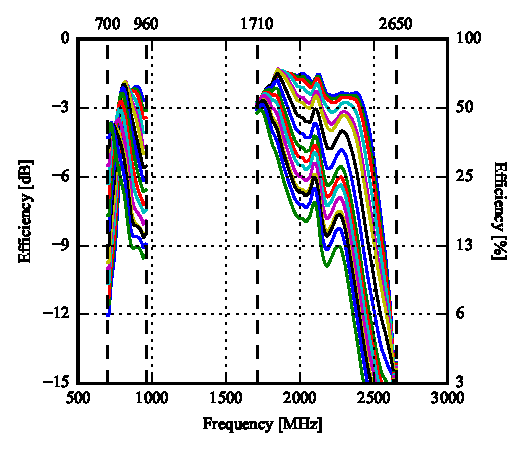
\includegraphics{img/tech_sol/monopole/highband/meas/final_tuner/efficiency_top.pdf}
        \caption{Top antenna.}
    \end{subfigure}
    \hfill
    \begin{subfigure}{0.49\linewidth}
        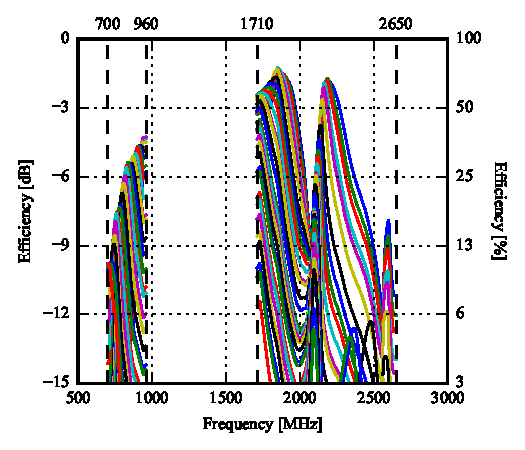
\includegraphics{img/tech_sol/monopole/highband/meas/final_tuner/efficiency_side.pdf}
        \caption{Side antenna.}
    \end{subfigure}
    \caption{Total efficiency of the final antenna design. The top antenna is swept from approximately \SI{0.6}{pF} to \SI{6}{pF} and the side antenna from approximately \SI{1.2}{pF} to \SI{12}{pF}. The tuners are tracking the first half of the sweep.}
    \label{fig:final_efficiency}
\end{figure}

\begin{table}
    \centering
    \begin{tabular}{|l|l|r|r|r|}
        \hline
        Antenna & Band & Start [MHz] & Stop [MHz] & Bandwidth [MHz] \\
        \hline
        Top & Low & 828 & 958 & 130 \\
        Side & Low & 935 & 1010 & 75 \\
        \hline
        Top & High    & 1773 & 2414 & 641 \\
        Side & High 1 & 1815 & 1980 & 165 \\
        Side & High 2 & 2166 & 2262 &  96 \\
        \hline
    \end{tabular}
    \caption{Maximum measured \SI{-6}{dB} impedance bandwidth of the final antenna design.}
    \label{tab:final_bandwidths}
\end{table}

%%%%%%%%%%%%%%%%%%%%%%%%%%%%%%%%%%%%%%%%%%%%%%%%%%%%%%%%%%%%%%%%%%%%%%%%%%%%%%%%
% Henrik og Lasse: I skal under ingen omstændigheder kopiere teksten nedenfor.
% Der går noget galt hvis I prøver! Skriv noget fra bunden i stedet!
%%%%%%%%%%%%%%%%%%%%%%%%%%%%%%%%%%%%%%%%%%%%%%%%%%%%%%%%%%%%%%%%%%%%%%%%%%%%%%%%

The measured S-parameters are shown in Figure~\ref{fig:final_sparams}. For the top antenna, the tunable bandwidth in the low band (by \SI{960}{MHz}) is \SI{130}{MHz} and can be swept all the way down to \SI{700}{MHz}. The high band can be covered from \SI{1710}{MHz} to around \SI{2450}{MHz}. There is still a problem covering the band from \SI{2550}{MHz} to \SI{2650}{MHz} but all bands from \SI{700}{MHz} to \SI{2400}{MHz} can be covered. For the side antenna, the tunable bandwidth by \SI{960}{MHz} is \SI{75}{MHz} and can be swept all the way down to \SI{700}{MHz}. The high band covers from \SI{1710}{MHz} to \SI{1975}{MHz} and from \SI{2095}{MHz} to \SI{2275}{MHz}. The impedance bandwidths are summarized in Table~\ref{tab:final_bandwidths}.

The measured efficiency is shown in Figure~\ref{fig:final_efficiency}. The top antenna is able to cover the low band at \SI{-4}{dB} efficiency and the high band at \SI{-3}{dB} from \SI{1710}{MHz} to \SI{2430}{MHz}. The side antenna is not as good and is only able to cover the low band at and efficiency between \SI{-10}{dB} to \SI{-4}{dB}. The high band has two resonances and is covered at \SI{-3}{dB} from \SI{1710}{MHz} to \SI{1960}{MHz} and from \SI{2130}{MHz} to \SI{2260}{MHz}. Both shown a problem covering the very highest bands above \SI{2550}{MHz}.

%%%%%%%%%%%%%%%%%%%%%%%%%%%%%%%%%%%%%%%%%%%%%%%%%%%%%%%%%%%%%%%%%%%%%%%%%%%%%%%%
%%%%%%%%%%%%%%%%%%%%%%%%%%%%%%%%%%%%%%%%%%%%%%%%%%%%%%%%%%%%%%%%%%%%%%%%%%%%%%%%

From the measurements it is seen that the top antenna is performs well in all bands except the bands from \SI{2550}{MHz} to \SI{2650}{MHz}. The side antenna does not perform quite as good but is piecewise acceptable -- especially in the high bands.
